\subsection*{\textit{\textbf{RQ3: Did the change in the release strategy have an impact on
the characteristics of delayed issues?}}}

\begin{sloppypar}
\noindent\textit{\textbf{Observation~5---Our models achieve a Brier score of 0.05-0.16 and ROC
areas of 0.81-0.83.}}\observation{obs:5}
The models that we fit to traditional releases achieve a Brier score of 0.16 and
an ROC area of 0.83, while the models that we fit to the rapid release data
achieve a Brier score of 0.05 and an ROC area of 0.81. Our models outperform
na\"{i}ve approaches such as random guessing and ZeroR---our ZeroR models
achieve ROC areas of 0.5 and Brier scores of 0.06 and 0.45 for rapid and
traditional releases, respectively. Moreover, the bootstrap-calculated optimism
is less than 0.01 for both the ROC areas and Brier scores of our models. This
result shows that our regression models are stable enough to perform the
statistical inferences that follow.\\

\begin{table}[t]
	\scriptsize
	\begin{center}
		\caption{Overview of the regression model fits. The $\chi^2$ of
		each metric is shown as the proportion in relation to the total
	$\chi^2$ of the model.  \label{tbl:regression_models} }
		%\resizebox{\textwidth}{!}{
			\begin{tabular}{cccc}
			\cline{3-4} 
			\multicolumn{2}{c}{} & 
			Traditional releases &
			Rapid releases 
			\tabularnewline
			\hline 
			\multicolumn{2}{c}{\# of instances} & 
			$34,673$ &
			$37,441$  
			\tabularnewline
			\hline
			\multicolumn{2}{c}{Wald $\chi^2$} & 
			$4,964$ &
			$2,705$  
			\tabularnewline
			\hline 
			\multicolumn{2}{c}{Budgeted Degrees of Freedom} &
			$1033$ & 
			$149$ 
			\tabularnewline
			\hline
			\multicolumn{2}{c}{Degrees of Freedom Spent} &
			$26$ & 
			$25$ 
			\tabularnewline
			%\hline 
			%\hline 
			%&  &  &  
			%\tabularnewline
			\hline 
			\multirow{2}{*}{Reporter experience} & 
			D.F. & 
			$1$ & 
			$1$  
			\tabularnewline 
			& 
			$\chi^2$ & 
			$2^{\ast\ast\ast}$ &  
			$2^{\ast\ast\ast}$ 
			\tabularnewline
			\hline 
			\multirow{2}{*}{Reporter integration} & 
			D.F. & 
			$1$ & 
			$1$  
			\tabularnewline 
			& 
			$\chi^2$ & 
			$5^{\ast\ast\ast}$ &  
			$4^{\ast\ast\ast}$ 
			\tabularnewline
			\hline 
			\multirow{2}{*}{Resolver Experience} & 
			D.F. & 
			$1$ & 
			\multirow{2}{*}{$\oslash$}
			\tabularnewline &
			$\chi^2$ & 
			$1^{\ast\ast\ast}$ &
			\tabularnewline 
			\hline 
			\multirow{2}{*}{Resolver integration} & 
			D.F. & 
			$1$ & 
			$1$  
			\tabularnewline 
			& 
			$\chi^2$ & 
			$2^{\ast\ast\ast}$ &  
			$5^{\ast\ast\ast}$ 
			\tabularnewline
			\hline 
			\multirow{2}{*}{Fix time} & 
			D.F. & 
			1 &
			1  
			\tabularnewline & 
			$\chi^2$ &
			$2^{\ast\ast\ast}$ &
			$8^{\ast\ast\ast}$ 
			\tabularnewline \hline 
			\multirow{2}{*}{Severity} &
			D.F. & 
			$6$ & 
			$6$ 
			\tabularnewline & 
			$\chi^2$ & 
			$1^{\ast\ast\ast}$ &  
			$1^{\ast\ast\ast}$  
			\tabularnewline \hline 
			\multirow{2}{*}{Priority} & 
			D.F. & 
			$5$ & 
			$5$ 
			\tabularnewline & 
			$\chi^2$ & 
			$1^{\ast\ast\ast}$ &  
			$\approx 0$   
			\tabularnewline \hline 
			\multirow{2}{*}{Size of description} & 
			D.F. & 
			$1$ &
			$1$  
			\tabularnewline & 
			$\chi^2$ & 
			$\approx 0$ &
			$1^{\ast\ast\ast}$   
			\tabularnewline \hline 
			\multirow{2}{*}{Stack trace attached} & 
			D.F. & 
			$1$ &
			$1$  
			\tabularnewline & 
			$\chi^2$ & 
			$\approx 0$ &  
			$\approx 0$ 
			\tabularnewline \hline 
			\multirow{2}{*}{Number of files} & 
			D.F. & 
			$1$ & 
			$1$
			\tabularnewline & 
			$\chi^2$ & 
			$1^{\ast\ast\ast}$ &  
			$1^{\ast\ast\ast}$ 
			\tabularnewline \hline 
			\multirow{2}{*}{Number of comments} & 
			D.F. & 
			$1$ &
			$1$ 
			\tabularnewline & 
			$\chi^2$ & 
			$\approx 0^{\ast}$ &  
			$31^{\ast\ast\ast}$  
			\tabularnewline \hline 
			\multirow{2}{*}{Number of tossing} & 
			D.F. & 
			$1$ &
			$1$  
			\tabularnewline & 
			$\chi^2$ & 
			$\approx 0^{\ast\ast\ast}$ &  
			$\approx 0$   
			\tabularnewline \hline 
			\multirow{2}{*}{Number of activities} & 
			D.F. & 
			$1$ &
			$1$  
			\tabularnewline & 
			$\chi^2$ & 
			$1^{\ast\ast\ast}$ &  
			$3^{\ast\ast\ast}$  
			\tabularnewline \hline 
			\multirow{2}{*}{Interval of comments} & 
			D.F. & 
			\multirow{2}{*}{$\oslash$} &
			\multirow{2}{*}{$\oslash$}  
			\tabularnewline &
			$\chi^2$ &
			&
			\tabularnewline \hline 
			\multirow{2}{*}{Code churn} & 
			D.F. & 
			$1$ & 
			$1$  
			\tabularnewline &
			$\chi^2$ &
			$\approx 0$ &  
			$\approx 0$ 
			\tabularnewline \hline 
			\multirow{2}{*}{Queue position} & 
			D.F. & 
			$1$ &             
			$1$
			\tabularnewline & 
			$\chi^2$ & 
			$17^{\ast\ast\ast}$ & 
			$2^{\ast\ast\ast}$
			\tabularnewline \hline 
			\multirow{1}{*}{Queue rank} & 
			D.F. & 
			$1$ & 
			$1$ 
			\tabularnewline &
			$\chi^2$ & 
			$56^{\ast\ast\ast}$ & 
			$14^{\ast\ast\ast}$
			\tabularnewline \hline 
			\multirow{2}{*}{Cycle queue rank} & 
			D.F. & 
			$1$ &
			$1$ 
			\tabularnewline &
			$\chi^2$ & 
			$10^{\ast\ast\ast}$ &
			$28^{\ast\ast\ast}$ 
			\tabularnewline \hline 
			\multirow{2}{*}{Cycle queue position} & 
			D.F. & 
			\multirow{2}{*}{$\oplus$} &
			\multirow{2}{*}{$\oslash$}  
			\tabularnewline &
			$\chi^2$ & 
			&
			\tabularnewline \hline 
		\end{tabular}
%	}
	\captionsetup{justification=centering}
	\caption*{
		$\oslash$ discarded during correlation analysis \\
		$\oplus$ discarded during redundancy analysis \\
		$\ast$ $p < 0.05$;
		$\ast\ast$ $p < 0.01$;
		$\ast\ast\ast$ $p < 0.001$\\ 
	}
	\end{center}
\end{table}

\noindent\textit{\textbf{Observation~6---Traditional releases prioritize the
delivery of backlog issues, while rapid releases prioritize the delivery
of issues of the current release cycle.}}\observation{obs:6}
\hyperref[tbl:regression_models]{Table}~\ref{tbl:regression_models} shows the explanatory power ($\chi^2$) of each
metric that we use in our models.  The \textit{queue rank} metric is the most
important metric in the models that we fit to the traditional release data.
Queue rank measures the moment when an issue is addressed in the backlog of the
project (see \hyperref[tbl:factors2]{Table}~\ref{tbl:factors2}).
\hyperref[fig:rankposition]{Figure}~\ref{fig:rankposition} shows the relationship that queue rank shares with
delivery delay. Our models reveal that the addressed issues in traditional
releases have a higher likelihood of being delayed if they are addressed later
when compared to other issues in the backlog of the project.   

\begin{figure}[t]
	\centering
	\subfloat{
		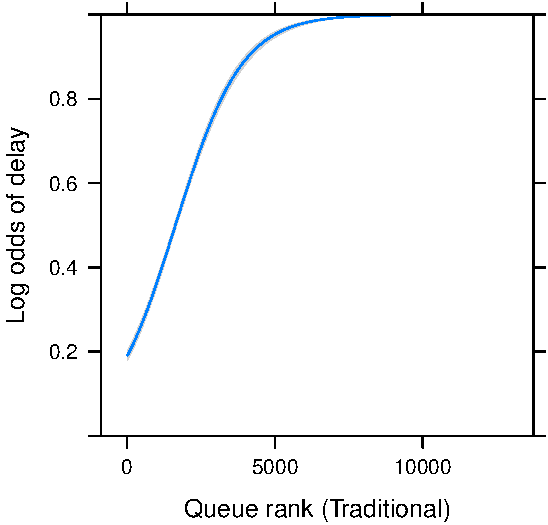
\includegraphics[width=0.43\textwidth,keepaspectratio]
		{chapters/chapter5/figures/rq3/queue_rank.pdf}
		\label{fig:rankposition}
	}
	\subfloat{
		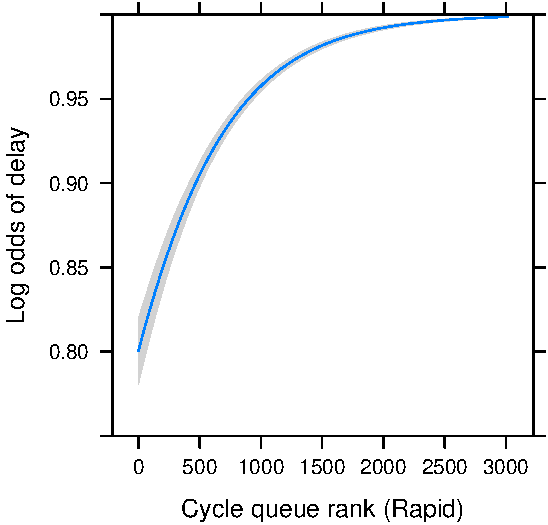
\includegraphics[width=0.43\textwidth,keepaspectratio]
		{chapters/chapter5/figures/rq3/cycle_queue_rank.pdf}
		\label{fig:cycle_rank}
	}

	\subfloat{
		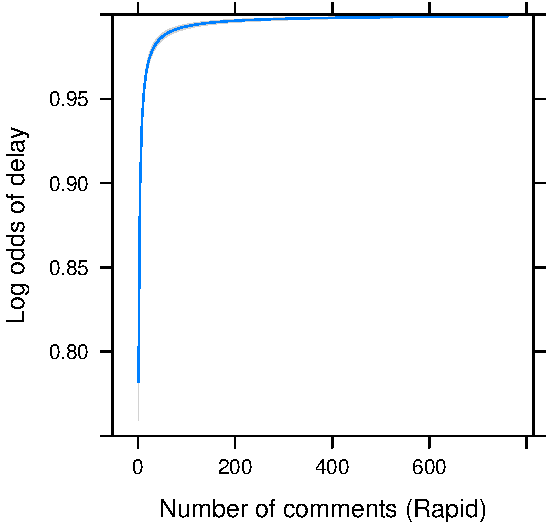
\includegraphics[width=0.43\textwidth,keepaspectratio]
		{chapters/chapter5/figures/rq3/comments.pdf}
		\label{fig:number_comments}
	}
	\caption{The relationship between metrics and delivery delay. The blue
		line shows the values of our model fit, whereas the grey
		area shows the 95\% confidence interval based on models fit to
		1,000 bootstrap samples. The parentheses indicate the
		release strategy to which the metric is related.
	}
\end{figure}

\begin{figure}[!]
	\centering
	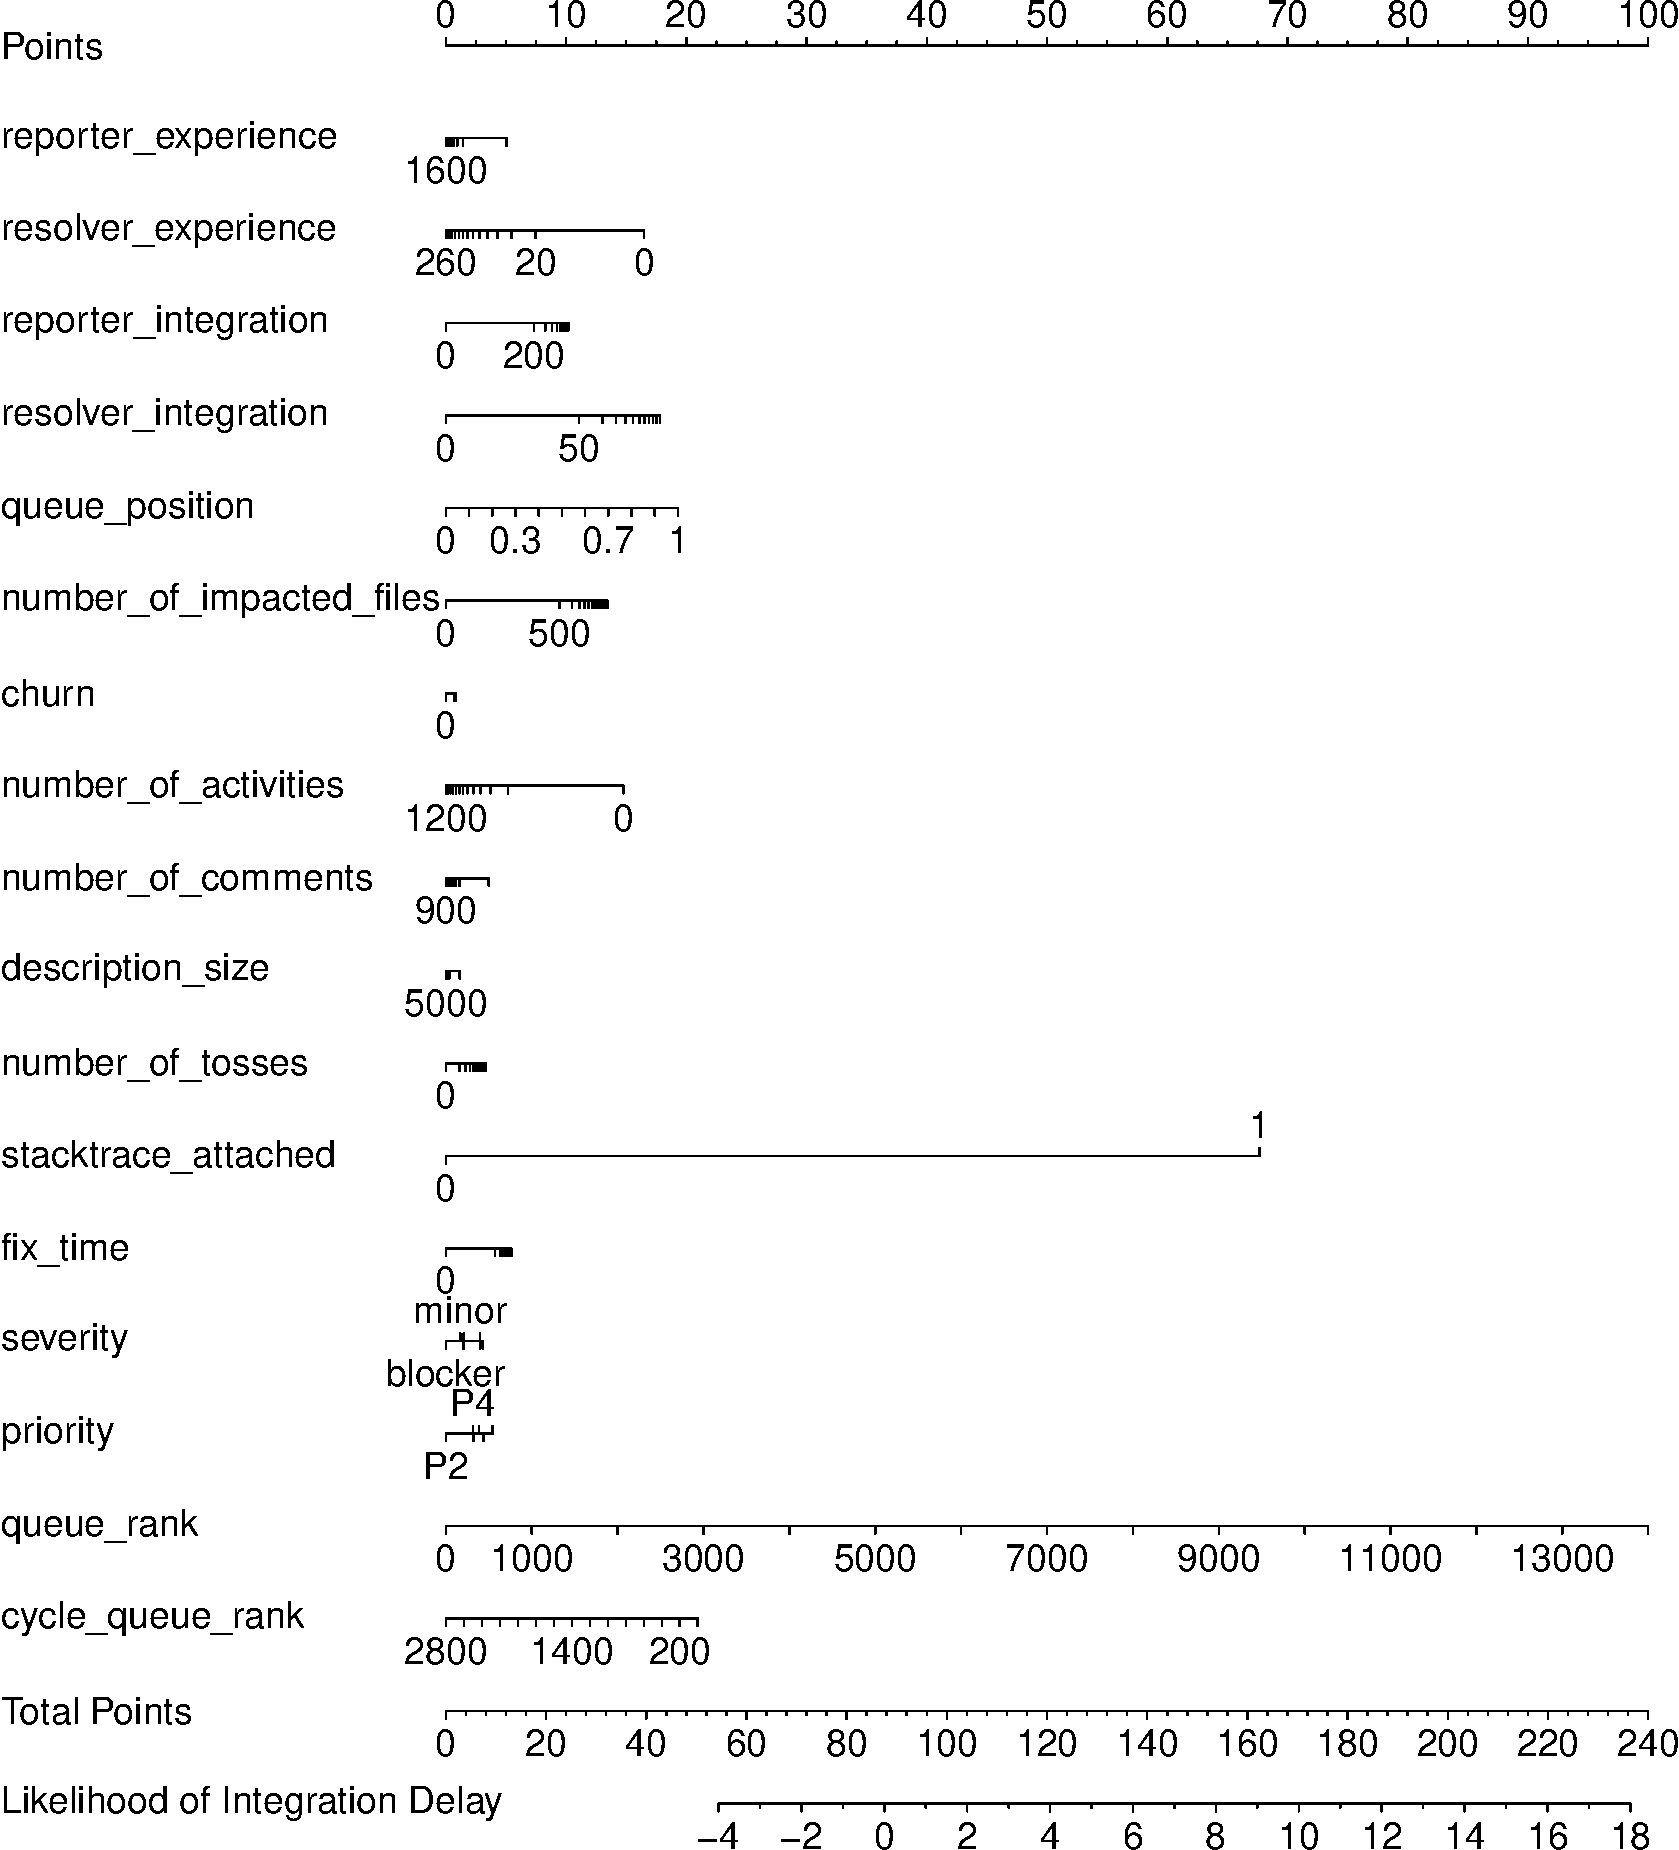
\includegraphics[width=0.90\textwidth,keepaspectratio]
	{chapters/chapter5/figures/rq3/nomogram_trad.pdf}
	\caption{Nomogram of our explanatory models for the traditional release cycle.}
	\label{fig:nomogram_trad}
\end{figure}

\begin{figure}[!]
	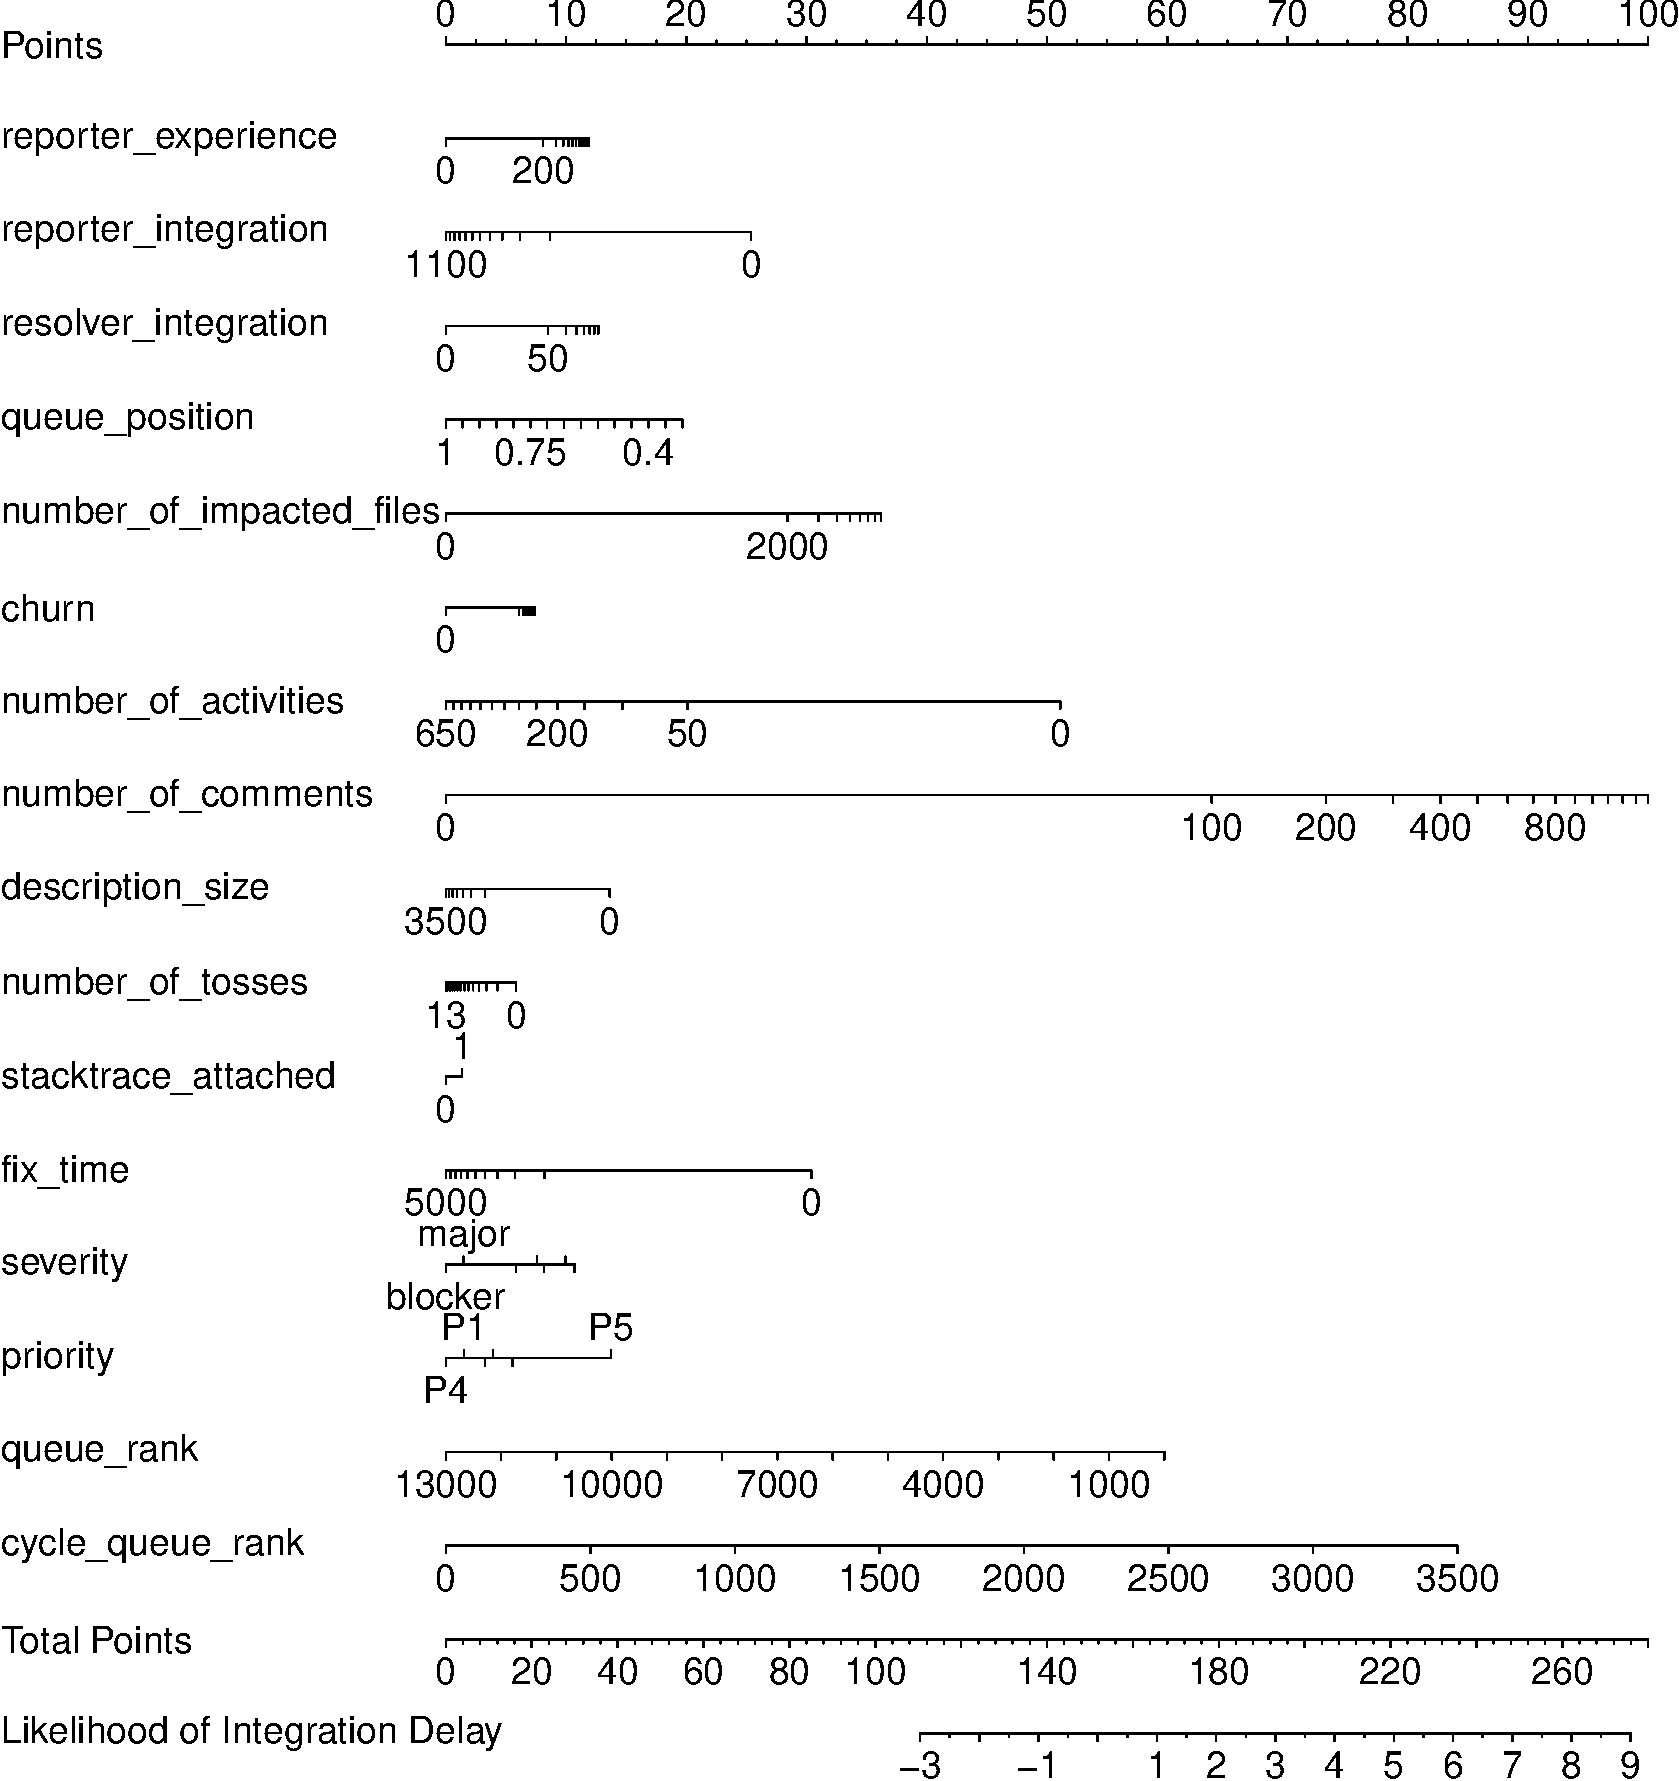
\includegraphics[width=0.90\textwidth,keepaspectratio]
	{chapters/chapter5/figures/rq3/nomogram_rapid.pdf}
	\caption{Nomogram of our explanatory models for the rapid release cycle.}
	\label{fig:nomogram_rapid}
\end{figure}

On the other hand, \textit{cycle queue rank} is the second-most important metric
in the models that we fit to the rapid release data. Cycle queue rank is the
moment when an issue is addressed in a given release cycle.
\hyperref[fig:cycle_rank]{Figure}~\ref{fig:cycle_rank} shows the relationship that cycle queue rank shares
with delivery delay. Our models reveal that the addressed issues in rapid
releases have a higher likelihood of being delayed if they were addressed later
than other addressed issues in the \textit{current release cycle}.
Interestingly, we observe that the most important metric in our rapid release
models is the \textit{number of comments}.
\hyperref[fig:number_comments]{Figure}~\ref{fig:number_comments}
shows the relationship that the \textit{number of comments} shares with
delivery delay. We observe that the greater the number of comments of an
addressed issue, the greater the likelihood of delivery delay. This result
corroborates the intuition that a lengthy discussion might be indicative of a
complex issue, which may be more likely to be delayed.

Moreover,
\hyperref[fig:nomogram_trad]{Figures}~\ref{fig:nomogram_trad}~and~\ref{fig:nomogram_rapid}
show the estimated effect of our metrics using
nomograms~\cite{iasonos2008build}. Indeed, our nomograms reiterate the large
impact of \textit{number of comments} (100 points) and \textit{cycle queue rank}
(84 points) in rapid releases, and the large impact of \textit{queue rank} (100
points) in traditional releases.  We also observe that \textit{stack trace
attached} has a large impact on traditional releases (68 points) despite not
being a significant contributor to the fit of our models (\cf
\hyperref[tbl:regression_models]{Table}~\ref{tbl:regression_models}). The large impact shown in our nomogram for
\textit{stack trace attached} is due to the skewness of our data---only $5$
instances within the traditional release data have the \textit{stack trace
attached} set to true. Thus, \textit{stack trace attached} cannot significantly
contribute to the overall fit~of~our~models.

Another \textit{key} difference between traditional
and rapid releases is how addressed issues are prioritized for delivery.
Traditional releases are analogous to a queue in which the earlier an issue is
addressed, the lower its likelihood of delay. On the other hand, rapid
releases are analogous to a stack of cycles, in which the earlier an issue is
addressed in the current cycle, the lower its likelihood of delay.\\
\end{sloppypar}

\conclusionbox{Issues that are addressed early in the
	project backlog are less likely to be delayed in traditional releases.
	On the other hand, issues in rapid releases are queued up on a per
	release basis, in which issues that are addressed early in the release
cycle of the current release are less likely to be delayed.}

